W przeciągu ostatniego ćwierćwiecza wynaleziono wiele technik oraz systemów służących do celów nawigacji: systemy satelitarne, systemy inercjalne,
systemy wizyjne oparte na przetwarzaniu obrazów cyfrowych w czasie rzeczywistym, radary wszelkiego typu.
Według panów Wan oraz Liu pojedynczy system dostarcza tylko częściowej informacji o środowisku zewnętrznym \cite[][strona 770]{CCTA_769_775}.
Ponadto dysponując tylko jednym narzędziem nie jest możliwa ocena jego wiarygodności. Z punktu widzenia statystyki matematycznej,
wiarygodność systemu, narzędzia, miernika jesteśmy w stanie określić wtedy i tylko wtedy gdy dysponujemy przynajmniej trzema niezależnymi od siebie źródłami danych.
Wtedy wykluczamy z opracowania błędne dane wejściowe. Ponadto im więcej posiadamy obserwacji danej wielkosći fizycznej tym większą jestesmy w stanie uzyskać dokładność.
Zatem pośrednio wyższa jest dokładność wyznaczenia pozycji oraz innych parametrów nawigacyjnych (kątowych)
w rozwiązaniach opartych na więcej niż jednym niezależnym źródle danych. W związku z powyższym systemy nawigacyjne oparte na fuzji obserwacji
pochodzących z kilku sensorów oraz systemów satelitarnych coraz bardziej zyskują na popularności \cite[][strona 770]{CCTA_769_775}
i prawdopodobnie w niedalekiej przyszłości zaczną dominować na rynku.
Pojedyncze obserwacje pochodzące z systemów GNSS charakteryzują się niską zmiennością ich dokładności w czasie.
Błąd wyznaczenia pozycji w przypadku rozwiązań kodowych pozostaje na niemalże stałym poziomie. 
W przypadku rozwiązań fazowych sytuacja jest podobna przy załorzeniu, że nie mamy utraty tzw. cykli fazowych.
Jeżeli jednak odbiornik utraci chociaż na moment sygnał do satelity, dokładność rozwiązania pogarsza się.
Nie spada jednak nigdy poniżej dokładności rozwiązania kodowego. Z teorii wynika,
że obserwacje GNSS charakteryzują się mniejszą rozdzielczością czasową niż obserwacje INS,
ponadto mogą występować miejscowe pogorszenia dokładności lub w ekstremalnych przypadkach brak rozwiązania.
%- trzeba porównać charakterystyki szeregów czasowych z ciekawych danych INS vs GNSS
%GNSS – raczej nie wystepuja bledy systematyczne – brak dryftu, czasami dziury w rozwiazaniach, gorsza rozdzielczośc pomiarow. 
%INS – dryft który narasta w czasie, wysoka rozdzielczosc pomiarow, brak dziór w obserwacjach,
%Wniosek – integracja tych dwoch systemow jest super:)
%TODO trzeba tutaj rysunek wstawic :)
\section{Zintegrowane systemy pozycjonowania w czasie rzeczywistym}
\subsection{Zastosowanie GNSS w precyzyjnym nawożeniu gleby}
W artykule \cite{CCTA5_188_192} panowie Guobing Pan oraz Xiao Feng opisują zastosowanie zintegrowanego systemu bazującego na  systemie GPS w precyzyjnym nawozeniu roślin.
Nawożenie ma czterdziesto procentowy wpływ na wielkość plonowania. Ponadto szalenie ważny jest stopień wykorzystania dawki nawozu przez rośliny.
Dawkowanie nawozów charakteryzuje się zmiennością czasową związaną z różnymi etapami wzrostu rośliny oraz zmiennością przestrzenną w obrębie danego pola \cite{CCTA5_188_192}.
Zbyt niski współczynnik wykorzystania nawozu przez rośliny uprawne prowadzi do wzrostu kosztów produkcji 
oraz negatywnie wpływa na środowisko poprzez zanieczyszenie wód gruntowych.
W związku z powyższym  zmienny rozkład przestrzenny nawożenia wydaje się kluczowy do osiagnięcia wymiernych korzyści ekonomicznych \cite{CCTA5_188_192}.
Wedug autorów artykułu maszyny rolnicze powinny poruszać się według uprzednio zaprojektowanej trasy w celu automatyzacji oraz zwiększenia wydajności nawożenia.
Do realizacji systemu precyzyjnego nawożenia panowie Pan oraz Xiao za priorytet obrali minimalizację kosztów.
System zatem bazuje na kodowych obserwacjach GPS, które są zintegrowane za pomocą filteracji Kalmana
z azymutem pochodzącym z elektronicznego kompasu oraz z danymi z precyzyjnych akcelerometrów oraz z żyroskopów.
Zaprojektowany system najpierw na podstawie psełdoodległości GPS oblicza współrzędne w układzie WGS-84,
następnie transformuje uzyskaną pozycję do współrzędnych płaskich w odwzorowaniu Gaussa-Krugera.
Następnie na pdstawie danych z żyroskopu oraz kompasu elektronicznego otrzymujemy najbardziej prawdopodobny azymut.
Powyższe dane poddawane są następnie poddane obrubce filtrem Kalmana w celu obliczenia ostatecznej pozycji oraz orientacji pojazdu w przestrzeni.
Aktualna pozycja pojazdu oraz orientacja przestrzenna jest następnie wykorzystywana w celu obliczenia punktowej dawki nawozu
oraz korekty potrzebnej systemowi sterowania do prowadzenia według zadanej ścieżki.

%---Zbieranie danych o glebie i jej właściwościach na potrzeby systemu precyzyjnego dawkowania nawozów 
%opartego na technologi GIS przy użyciu systemu pozycjonowania GPS (DGPS, RTK)
\indent Systemy nawigacji satelitarnej pomagają w zwiększeniu rozdzielczości oraz dokładności danych przestrzennych
dla potrzeb systemu dawkowania nawozów. Obecnie szybka akwizycja danych terenowych opisujących właściwości glebowo rolnicze pól uprawnych
stanowi ważny aspekt badań nad rozwojem rolnictwa precyzyjnego. Zwiększenmie rozdzielczoąci prubkowania jest możliwe dzięki
dynamicznemu rozwojowi nawigacji w czasie rzeczywistym (RTK, DGPS) zwłaszcza poprzez lokalne systemy stacji referencyjnych ASG-EUPOS.
Dla przykładu im wyższa jest rozdzielczość prubkowania, tym dokładniejsza jest interpolacja danych 
(ph, fizyko chemiczne właściwości gleby itp, określana przez system GIS) na potrzeby określania dawek nawozów.
Posumowując: Dane przestrzwenne zbierane były za pomocą DGPS z wykorzystaniem lokalnych stacji referencyjnych.
Następnie wyniki pomiarów parametrów glebowych były wprowadzane do GIS-owej bazy danych.
Na podstawie zebranych danych były tworzone mapy nawożenia \cite{CCTA5_268_278}.

\subsection{Algorytmy wyznaczania pozycji oparte na filtrze Kalmana}
Prowadzenie równoległe jest jedną z najbardziej popularnych obecnie metod ułatwiających prace polowe.
W pracy \cite{CCTA5_461_469} czytamy, że przeprowadzono już wiele badań nad zastosowaniem bardzo dokładnych odbiorników fazowych RTK-GPS
przy automatyzacji maszyn rolniczych. Autorzy twierdzą jednak, że koszt precyzyjnych odbiorników GPS jest zbyt wysoki
i nie pozwala na ich powszechną adaptację w rolnictwie. Ponieważ, zintegrowane systemy nawigacyjne oparte na filtrze Kalmana
znacznie podnoszą dokładność pozycjonowania, a technologia czujników elektronicznych bardzo szybko się rozwija,
możliwa jest zatem konstrukcja tanich systemów pozycjonowania atrakcyjnych pod względem zastosowania ich w rolnictwie precyzyjnym \cite{CCTA5_461_469}.
Panowie Zhang, Feng, Li, Rao oraz Di Cui skonstruowali zintegrowany system do równoległego prowadzenia złożony z odbiornika DGPS,
z elektronicznych żyroskopów MEMS, z dwóch czujników prędkości oraz z precyzyjnego potencjometru do pomiaru skrętu kół.
Schemat blokowy omawianego systemu przedstawiono na rysunku \ref{fig:ch4_multisensorSystem}.
Dane z poszczególnych podzespołów przesyłane były do komputera z systemem wbudowanym na którym zainstalowano Filtr Kalmana.
Całkowity koszt systemu wyniósł w przybliżeniu około 1500\$.
\begin{figure}[H]
\centering
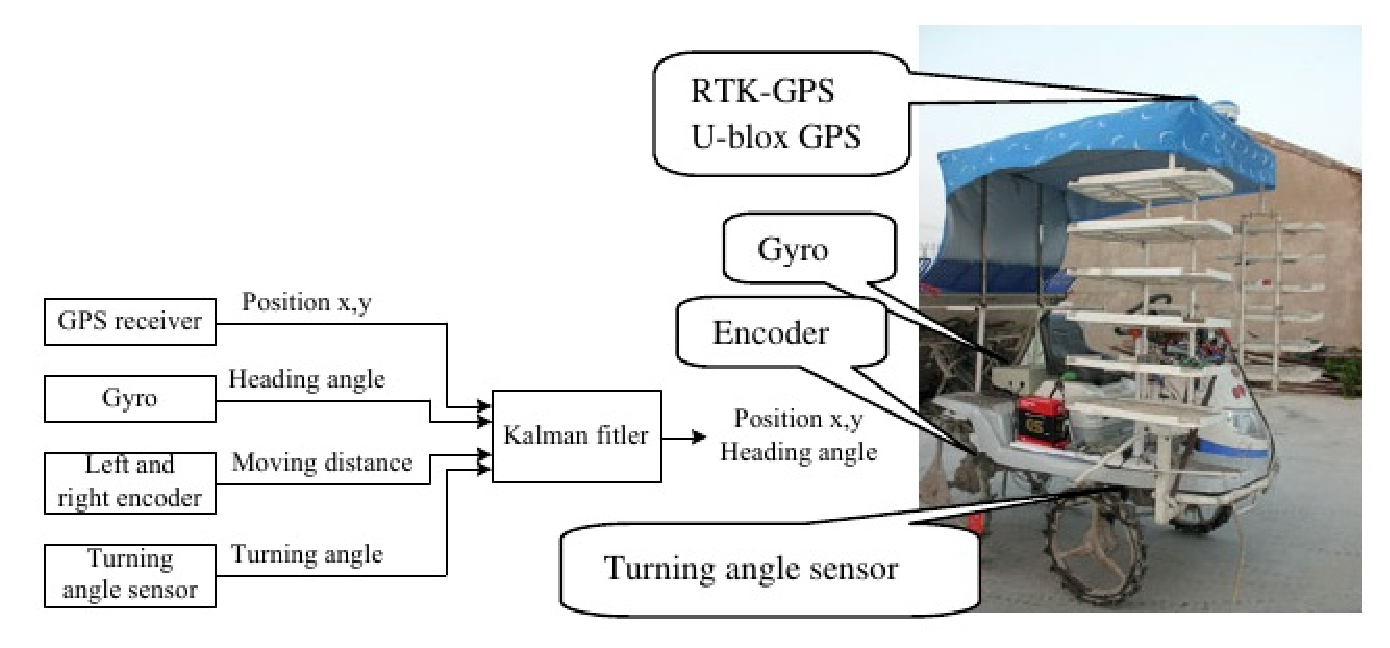
\includegraphics[width=\textwidth]{ch4_multisensorSystem.eps}
\caption{\textit{Przykład zintergrowanego systemu do równoległego prowadzenia;} 
źródło: \cite[][strona 464]{CCTA5_461_469}}
\label{fig:ch4_multisensorSystem}
\end{figure}   
RTK-GPS był używany jako odniesienie w celu porównania otrzymanych wyników. 
Współrzędne w lokalnym układzie odniesienia, azymut, oraz prędkość były zadane jako wektor stanu w filtrze Kalmana.
Wyniki eksperymentu pokazały, że obróbka danych przestrzennych za pomocą filtru Kalmana znacznie podnosi dokładność wspólrzędnych DGPS.
Średnie residua w odniesieniu do pozycji GNSS zostały zredukowane z 2.21m do 0.52m względem osi x oraz z 0.68m do 0.23m względem osi y.
Jednakże zaimplementowany algorytm nie usunął całkowicie błędów systematycznych zawartych w danych kodowych DGPS.
Maksymalna odchyłka od równoegłości po przebyciu 70 m wyniosła 3m \cite{CCTA5_461_469}.

\indent Kolejnym przykładem fuzji danych jest integracja danych RTK-GPS z elektronicznym kompasem oraz obrazowaniem cyfrowym z urzyciem logiki rozmytej (Fuzzy logic).
W artykule pod tytułem “Automatic Navigation System With Multiple Sensors” panowie Wan oraz Liu
opisali system automatycznego prowadzenia pojazdów rolniczych bazujący na integracji obserwacji pochodzących z elektronicznego kompasu,
odbiornika GPS oraz kamery cyfrowej z matrycą CCD. W celu obliczenia parametrów prowadzenia pojazdu względem zadanej trasy,
dane z wszystkich powyższych mierników były przetwarzane z użyciem narzędzi logiki rozmytej tzw. Fuzzy Logic.
Poniżej na rysunku nr \ref{fig:ch4_fuzzyLogic} przedstawiono diagram blokowy opisujący algorytm integracji danych.
\begin{figure}[H]
\centering
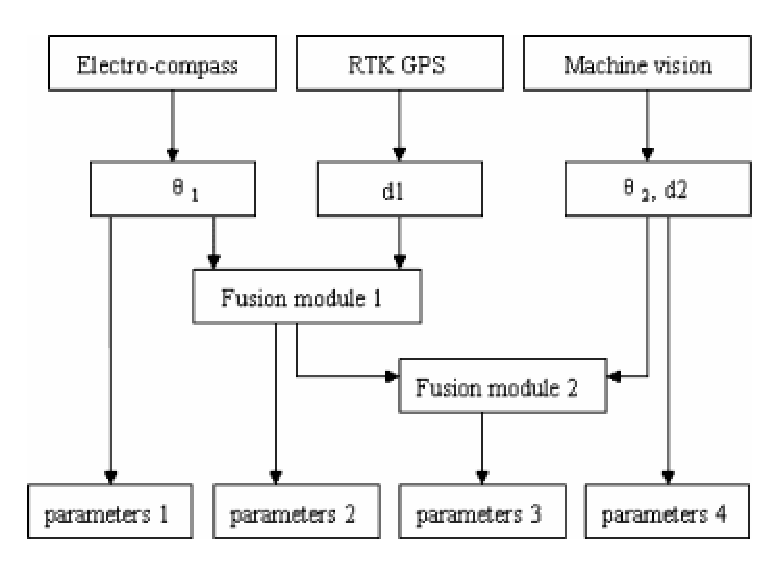
\includegraphics[width=7cm, height=6cm]{ch4_fuzzyLogic.eps}
\caption{\textit{Zastosowanie narzędzi logiki rozmytej do integracji danych nawigacyjnych;}
źródło: \cite[][strona 774]{CCTA_769_775}}
\label{fig:ch4_fuzzyLogic}
\end{figure}

Azymut kierunku jazdy względem zadanej ścieżki oraz ofset oznaczono odpowiednio jako $\theta$ oraz d.
Wszystkie powyższe rezultaty pośrednie zanim przesłano do modułów logiki rozmytej, przetransformowano do układu obrazu cyfrowego,
w celu zapewnienia jednolitego układu odniesienia. Jako ostateczną i najbardziej prawdopodobną wersję parametrów $(d, \theta )$
przyjęto wyniki z modułu numer 2 (parameters 3), pozostałe rezultaty posłużyły do wybrania jak najlepszych współczynników skalowania obserwacji
w modułach wykorzystujących logikę rozmytą. Na podstawie parametrów określających położenie pojazdu względem zdefiniowanej uprzednio trasy
obliczany był teoretyczny kąt skrętu kół, przekazywany następnie do realizacji w układzie sterującym (target angle), rysunek \ref{fig:ch4_fuzzyLogicTargetAngle}.
\begin{figure}[H]
\centering
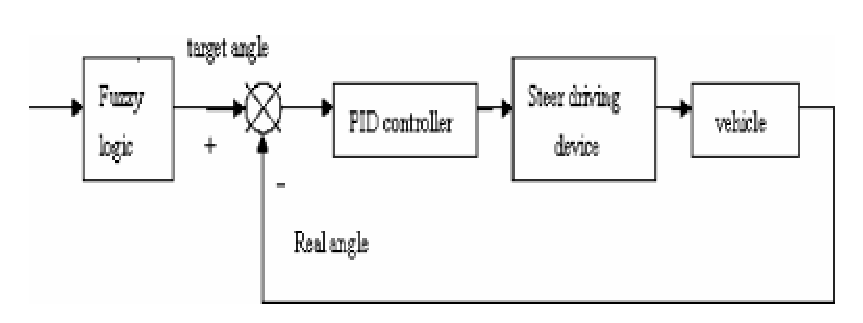
\includegraphics[height=4cm]{ch4_fuzzyLogicTargetAngle.eps}
\caption{\textit{Schemat algorytmu znajdującego odpowiedni kąt skrętu kół pojazdu rolniczego;}
	źródło: \cite[][strona 775]{CCTA_769_775}}
\label{fig:ch4_fuzzyLogicTargetAngle}
\end{figure}
System sterujący realizował swoje zadania w oparciu o algorytm PID - regulator proporcjonalno - całkująco - różniczkujący.
Według autorów pracy \cite{CCTA_769_775} opisany system spełnia wymagania automatycznego prowadzenia maszyn rolniczych w warunkach roboczych.
\section{Spegcjalistyczne opracowanie obserwacji - postprocessing}
Opracowanie obserwacji w trybie postrocessingu jest szczególnie ważne z punktu widzenia opracowania map plonowania.
Pan Xiaochao Zhang wraz z zespołem w artykule \cite{CCTA_951_958} opisali konstrukcję systemu służącego do tworzenia map plonowania.
Głównym elementem systemu był poziomo umieszczony czujnik mierzący masę przepływającego ziarna.
Surowe wyniki były poprawiane ze względu na wilgotność, a następnie zamieniane na ilość ziarna przez algorytm całkujący.
Mapa plonu była tworzona przy wykorzystaniu danych przestrzennych z odbiornika GPS, po uprzedniej synchronizacji czasowej.
W celu zwiększenia dokładności mapowania obserwacje GPS były poddane specjalistycznemu opracowaniu tzw. Postprocessing,
zanim zintegrowano je z danymi plonowania. Ostateczne wyniki podczas testów charakteryzowały się błędem względnym na poziomie 3.5\%. 
Poniższy rysunek \ref{fig:ch4_creatingPlantsMap} przedstawia działający system w trybie operacyjnym.
\begin{figure}[H]
\centering
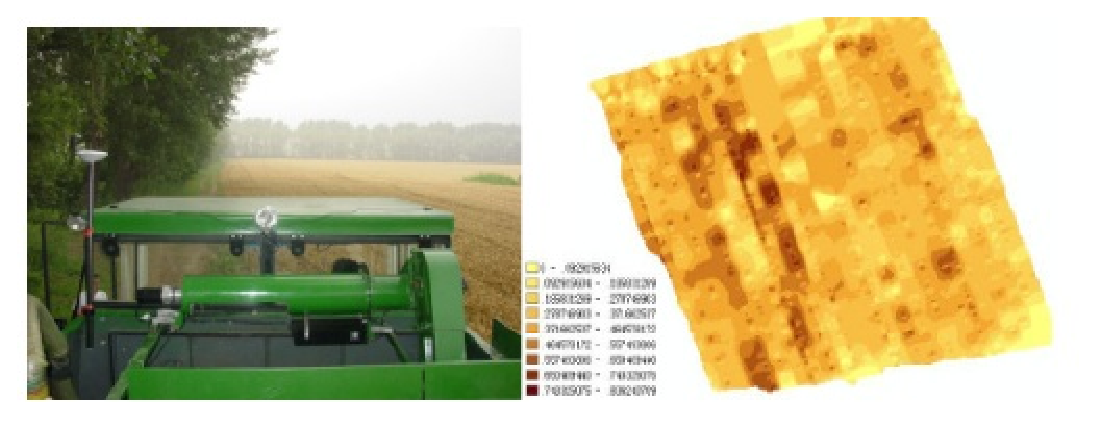
\includegraphics[width=\textwidth]{ch4_creatingPlantsMap}
\caption{\textit{System do tworzenia map plonowania;} źródło: \cite[][strona 954]{CCTA_951_958}}
\label{fig:ch4_creatingPlantsMap}
\end{figure}
Mapy plonów są ważnym źródłem informacji dla rolników. Pomagają w planowaniu zabiegów agrotechnicznych.

\section{Inne zastosowania GNSS w rolnictwie precyzyjnym}
%--- pomiary pól powierzchni na potrzeby rolnictwa precyzyjnego
%	( Computer and Computing Technologies in Agriculture; volume 2; s. 993)

%--- zastosowanie GPS w automatycznym zmiennym nawadnianiu 
Celem precyzyjnego nawadniania jest minimalizacja użycia zasobów wodnych, przy załorzeniu  spełnienia w jak największym stopniu wymagań roślin uprawnych.
Dystrybucja przestrzenna wymagań roślinnych względem ilości dodatkowego nawadniania, zależy głównie od warunków glebowych oraz topografii terenu.
Dlatego zasadnym jest przeprowadzanie nawadniania pól uprawnych, zgodnie z wcześniej sporządzanymi mapami docelowego rozkładu przestrzennego dawek H2O 
\cite{PA_RemoteIrrigation}.
\begin{figure}[H]
\centering
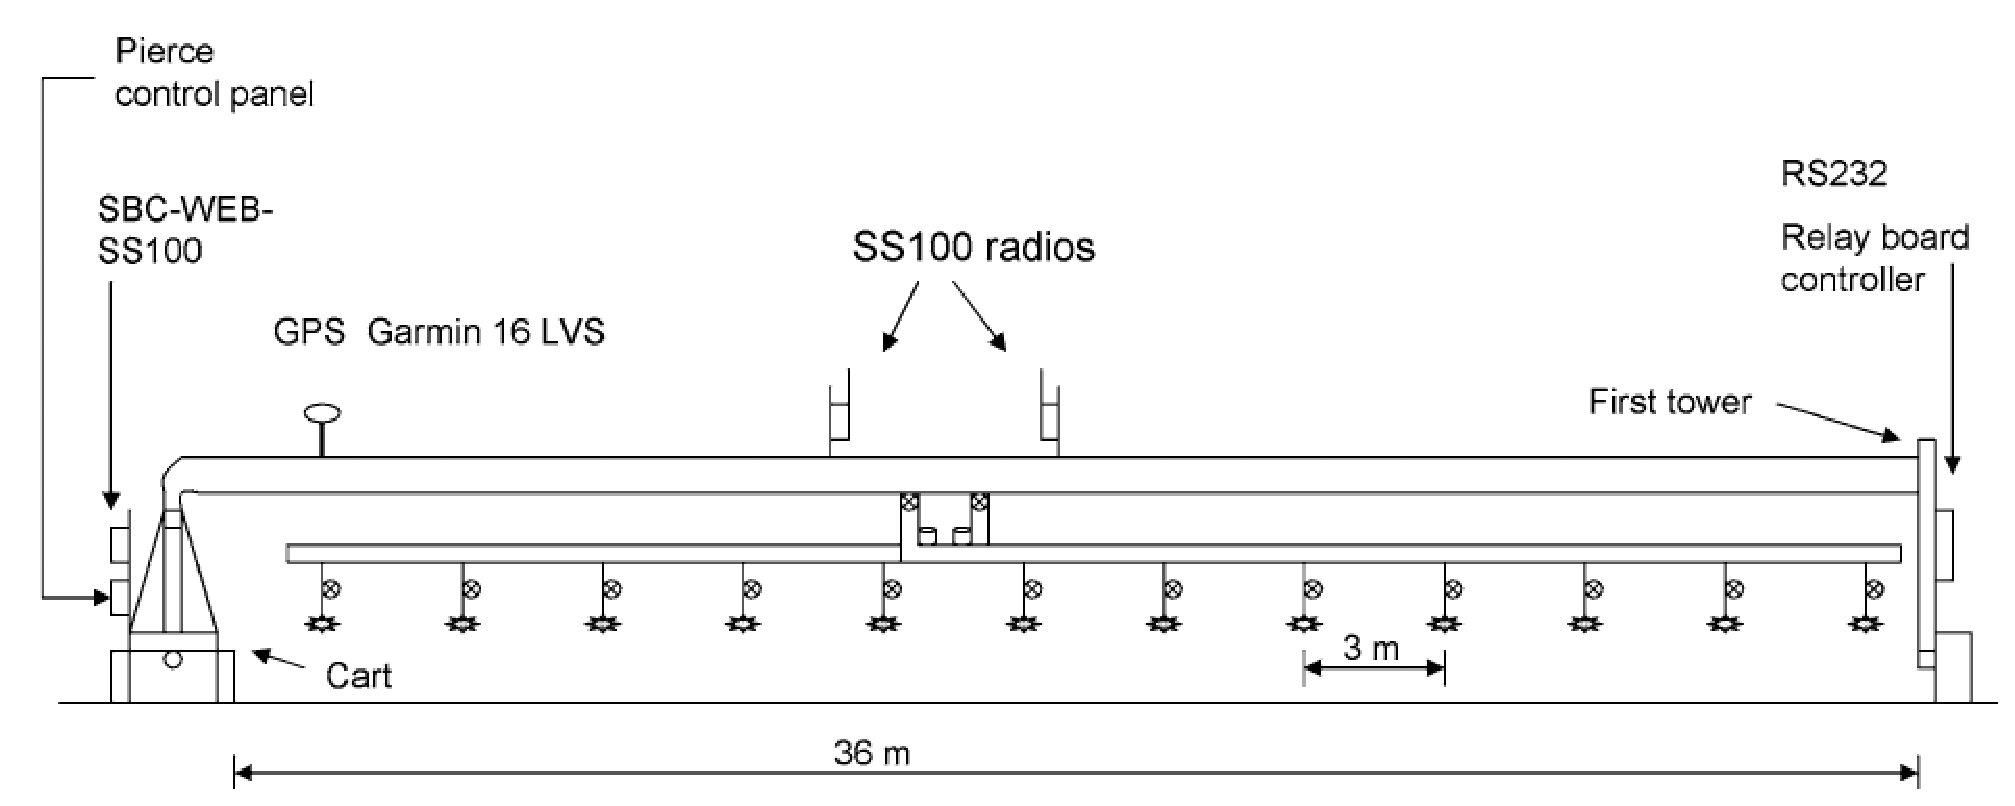
\includegraphics[width=\textwidth]{ch4_remoteIrigationMonitoring}
\caption{\textit{Schemat systemu służącego do automatycznego nawadniania pól uprawnych;} źródło: \cite[][strona 04]{PA_RemoteIrrigation}}
\label{fig:ch4_remoteIrigationMonitoring}
\end{figure}
Jose L. Chavez i wsp. w artykule \cite{PA_RemoteIrrigation} zaprojektowali system precyzyjnego nawadniania, sterujący niezależnie poszczególnymi dyszami,
których przepływ determinowano w oparciu o mapy nawadniania. Na rysunku \ref{fig:ch4_remoteIrigationMonitoring} przedstawiono schemat systemu.
Z punktu widzenia niniejszego opracowania najważniejszym elementem systemu jest odbiornik GPS umieszczony precyzyjnie nad pierwszą dyszą,
który pozwala na określenie jej pozycji przestrzennej i obliczenie dawki H2O. Położenie kolejnych dysz określano za pomocą translacji
o zadany wektor względem pierwszej, przy załorzeniu, że ramię systemu jest zawsze prostopadłe do kierunku ruchu.
Mapy nawadniania tworzone były na podstawie danych o wilgotności gleby oraz powietrza zbieranych za pomocą sieci czujników
równomiernie rozmieszczonych na polu uprawnym. 

